\chapter{Autonomous Energy Production for Isolated Site}
\textit{Note: The devices and sizing presented below are a simplified approach to the problem.}

The context is that of an isolated site that we want to power using photovoltaic (PV) panels and storage batteries.

The site consumes energy continuously with a "base" power and consumption peaks throughout the day.

To maintain operation during the night, energy storage by batteries is associated with the PV panels.

The energy supply is provided in alternating current, with a service voltage of 230 VAC - 50 Hz generated by a single-phase inverter.

The general architecture of the system is as follows:

\begin{figure}[h]
\centering
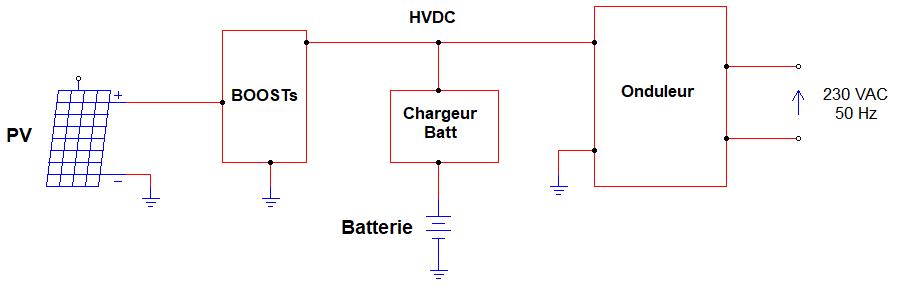
\includegraphics[width=0.8\linewidth]{TD_Boost_2Q_Onduleur/fig/Archi_Globale.png}
\caption{Overall architecture}
\end{figure}

\textbf{Main data}

\underline{Installation:}
\begin{itemize}
\item Base power of the installation: 300 W
\item Peak power consumption: 1500 W
\item Duration of power peaks: 3x30 min between 11:00 and 15:00.
\end{itemize}

\underline{PV panels:}
\begin{itemize}
\item The PV panels are oriented to the south, with an inclination of $35^\circ$. The installation is located in the Alps, south of Briançon, in a geographical area where the average annual irradiation is $1500\ kWh/m^2$ (taking into account shading).

\item The datasheet of a PV panel provides the following information:
\clearpage
\begin{centering}
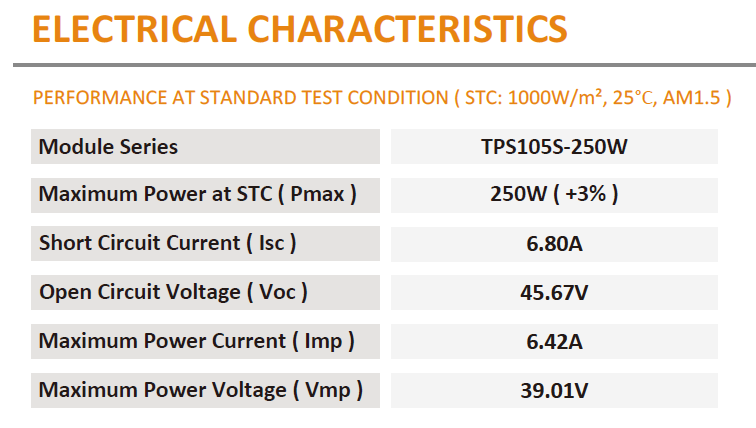
\includegraphics[width=0.49\linewidth]{TD_Boost_2Q_Onduleur/fig/elec_specif.png}
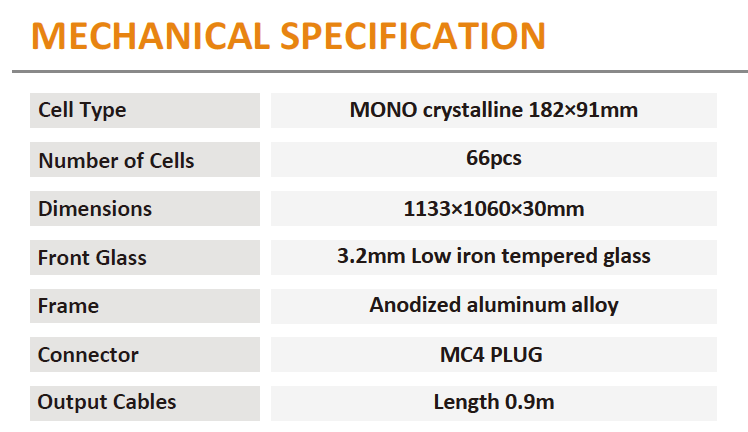
\includegraphics[width=0.49\linewidth]{TD_Boost_2Q_Onduleur/fig/meca_specif.png}
\end{centering}


\item The overall efficiency of the PV panels is 20\% (taking into account the ratio [cell area / total area]) and it is considered that the overall efficiency of the energy conversion chain is 90\% (including converters, line losses, etc.).
\end{itemize}



\section*{Preliminaries}
Determine:
\begin{enumerate}
\item The energy consumed by the installation per day and per year.
\item The required PV panel area to supply the system, taking into account the efficiencies.
\item The minimum number of PV panels required.
\end{enumerate}


\section{BOOST Converters}
\label{sec:Convertisseur_BOOST}

It is decided to implement \textbf{12 PV panels}, grouped in two series-connected PV panel groups. Each PV panel group is connected to an input of a BOOST DC-DC converter.
Thus, the developed structure of the "BOOST" in Figure 1 is as follows:

\begin{figure}[h]
\centering
\includegraphics[width=0.6\linewidth]{TD_Boost_2Q_Onduleur/fig/Archi_Boost.png}
\caption{Boost architecture}
\end{figure}

It is assumed that all PV panels are uniformly illuminated so that each PV panel group provides half of the instantaneous power consumed.

The HVDC output voltage is regulated at \textbf{500 V} by control loops acting on the duty cycles of transistors Q1 and Q2.

The switching frequency of Q1 and Q2 is fixed and equal to \textbf{Fd = 50 kHz}.

\underline{For now, we are only interested in BOOST 1 and we assume that all components are ideal.}

Considering that:
\begin{itemize}
\item The BOOST input voltage (on C1) and HVDC are rigorously constant over one switching period.
\item The ripple current $\Delta I$ in L1 represents 20\% of the average input current.
\item We are in continuous conduction mode.
\end{itemize}

\begin{enumerate}
\item Represent the currents in L1, Q1, and D1, as well as the voltages across them, over two switching periods and for a duty cycle of 50\%.

\item Determine the expression of HVDC as a function of the input voltage, denoted Vpv, and the duty cycle $\alpha$. Similarly, express the relationship between the input current Ipv (average current in L1) and the output current $I_{HVDC}$.

\item Determine literally:
\begin{enumerate}
\item The maximum voltage applied to the terminals of Q1 and D1.
\item The average and maximum values of the currents in L1, Q1, and D1 as a function of Ipv, $\Delta I$, and the duty cycle.
\item Summarize these results in a constraints table (useful for component selection).
\end{enumerate}

Now, consider both BOOST converters operating and sharing the power equally. The environmental conditions are STC conditions ($1000 W/m^2$ - $25^\circ C$).

We also consider an operating sequence in which (first extreme case):
\begin{itemize}
\item The power consumed by the load is maximum.
\item The battery is not fully charged and consumes the power difference between the power consumed by the load and the power supplied by the PV panels, which corresponds to the total "peak" power.
\end{itemize}

\item Determine:
\begin{enumerate}
\item The total power $P_{cT}$ that the PV panels can provide considering the irradiation.
\item The power flowing through each BOOST converter.
\item The power consumed by the battery.
\end{enumerate}

\item Under these operating conditions, for each of the two BOOST converters, determine:
\begin{enumerate}
\item The input voltage Vpv.
\item The input current Ipv.
\item The control duty cycle of the transistors.
\item The value of L for which $\Delta I$ represents 20\% of Ipv.
\item The constraints applied to the power components Q and D (maximum voltage, average and maximum current).
\end{enumerate}

Now, assume that the power consumed by the load is the minimum power and the battery is fully charged (second extreme case).

\item Suppose that the conditions are still STC conditions and that the output voltage of a PV panel is 44 V.
\begin{enumerate}
\item Determine the power supplied by each group of PV panels and the input current of each BOOST converter.
\item Are the BOOST converters still operating in continuous conduction mode?
\item Represent the input current in L and the voltage across it.
\item Express the input current Ipv as a function of Vpv, HVDC, L, Fd, and the transistor conduction time $t_{on}$.
\item Determine the new value of the duty cycle to maintain HVDC at 500 V.
\end{enumerate}

\end{enumerate}

\newpage
\section{Battery Charger (Half-Bridge)}

To provide electricity supply during the night, a battery pack is installed.

The power structure associated with the batteries is that of a reversible converter of the "Half Bridge" type (2-quadrant chopper). This converter allows powering the installation from the pack during the night and recharging the pack from the PV panels during the day.

\vspace{0.5cm}
The following diagram shows this structure:

 \begin{figure}[h]
\centering
\includegraphics[width=0.8\linewidth]{TD_Boost_2Q_Onduleur/fig/Archi_2Q.png}
\caption{2-quadrant chopper architecture}
\end{figure}


In all cases, the control loops of the BOOST and Half-Bridge converters maintain \textbf{HVDC = 500 V.}

The battery pack voltage is assumed to be constant and equal to \textbf{Ubatt = 120 V} (38 elements of 3.2 V / LiFePo4 technology).

A battery current limiting loop included in the BMS (Battery Management System) limits it to $I_{batt\_max} = 10\ A$.

Transistors Q3 and Q4 are driven in complementary control at a fixed frequency of 50 kHz. Dead times are neglected.

Hereafter, the duty cycle refers to the ratio of the conduction time of Q3 to the switching period.

\begin{enumerate}
\item For a given duty cycle (0.3 for example) and in continuous conduction mode, represent, for charge currents ($I_{L3} > 0$) and battery discharge currents of the same absolute values:
\begin{enumerate}
\item The currents in L3, Q3, and Q4.
\item The voltage across L3.
\item Indicate the directions of current flow in L3.
\end{enumerate}

\item Express the relationship between the battery voltage and HVDC as a function of the control duty cycle of Q3 denoted $\alpha_{HB}$ (in continuous conduction mode).

Initially, we are in the daytime while the pack is being charged in a configuration corresponding to question 4 of TD \ref{sec:Convertisseur_BOOST}. In this configuration, the battery charging current is $I_{batt\_max}$.

\item Is the Half-Bridge converter operating in "Buck" or "Boost" mode? What is the purpose of C3?

\item We want the ripple current in L3 to represent 30\% of its average current (i.e., 3 A). Determine:
\begin{enumerate}
\item The control duty cycle of Q3.
\item The value to be given to L3.
\end{enumerate}

\item For this operating point, determine the voltage, maximum current, and average current constraints on Q3 and Q4.

We are still in the daytime, but now in a configuration where the installation calls for its maximum power (1800 W). The weather conditions are such that the PV panels can only provide 1000 W (including Boost efficiencies).

\item What is the power supplied by the battery and what is its current?

\item Is the Half-Bridge operation "Buck" or "Boost"?

\item What is the control duty cycle of Q3? Is the HB converter still operating in continuous conduction mode? Represent the currents in L3, Q3, and Q4 and the voltage $V_{L3}$ indicating the remarkable numerical values. Provide the equivalent diagrams for the two operating phases indicating the directions of current flow.

\item During the night, the battery alone supplies power to the installation and the power consumed is 300 W. We assume that the HB efficiency is unity.
\begin{enumerate}
\item Determine the value of the control duty cycle of Q3 to maintain HVDC at \hbox{500 V}.
\item Represent the current in L3 indicating its average value.
\end{enumerate}

\item Taking into account a global efficiency of [HB + Inverter] of 90\%, what should be the minimum capacity (in Ah) of the pack to maintain autonomy for 16 consecutive hours with a maximum discharge rate of 90\% (during this period, the phases at maximum power do not occur).

\end{enumerate}

\newpage
\section{Single-Phase PWM Inverter on RL Load}

We now turn our attention to the single-phase inverter. The grid is modeled by an R-L load in series. The block diagram is as follows:

\begin{figure}[h]
\centering
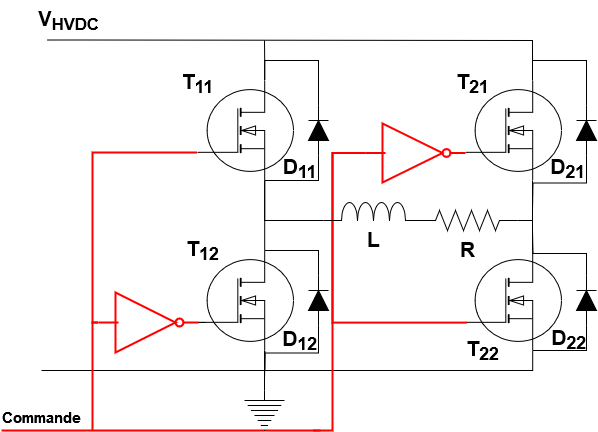
\includegraphics[width=0.8\linewidth]{TD_Boost_2Q_Onduleur/fig/Onduleur.png}
\end{figure}

\begin{itemize}
\setlength\itemsep{-1mm}
\item The transistors operate in PWM at a switching frequency $F_d$ much higher than the frequency of the output voltage to be reconstructed.
\item The duty cycle varies over time and will be denoted as $\alpha(t) = 0.5 + \delta_\alpha \sin(\omega t)$.
\end{itemize}



Hereafter, we refer to:

\begin{itemize}
\setlength\itemsep{-1mm}
\item $V_0$: the voltage across the $L - R$ combination (inverter output voltage).
\item $I_R$: the current in the R-L load.
\end{itemize}

The main characteristics of the load are:

\begin{itemize}
\setlength\itemsep{-1mm}
\item Equivalent circuit: series $R - L$, with $L = 30 mH$
\item Rated power: 1500 W
\item Rated voltage across $R$: $U_{Rn} = 230 V$ (rms value)
%\item After startup, the power absorbed by the load increases linearly from 300 to 500 W over 300 seconds, then stabilizes at 500 W.
%\item In the same time interval, the rms voltage across $R$ (denoted: $U_R$) increases linearly from 40 to 100 V.
\end{itemize}

\begin{enumerate}
%\item On the same graph, and during the 400 seconds following startup, represent the evolutions of:
%
%\begin{enumerate}
%\item the power absorbed by the load
%\item the voltage across $R$: $U_R$
%\item the rms current in the load $I_R$
%\end{enumerate}

\item Output voltage $V_0$

\begin{enumerate}
\item Represent the shape of the output voltage for a duty cycle $\alpha > 0.5$ over one switching period.
\item Express the average value of $V_o$ over one switching period as a function of the duty cycle $\alpha$ and $V_{DC}$.
\item Express the time-varying average value (over one switching period) of the output voltage $<V_0>(t)$ as a function of $V_{DC}$ and $\delta_\alpha$.
\item Determine the rms value of $<V_0>(t)$ (denoted $V_{0\ eff}$) as a function of $V_{HVDC}$ and $\delta_\alpha$.
\item Neglecting the current component due to switching, give the expression of the current in $R$ ($I_R(t)$) taking $<V_0>(t)$ as the reference phase.
\item Express the rms value of the current in $R$ as a function of $V_{0\ eff}$, $R$, $L$, and $\omega$.
\item Express the phase shift $\varphi$ between $I_R(t)$ and $<V_0>(t)$ as a function of $R$, $L$, and $\omega$.
\item Express the power factor of the RL load as a function of $R$, $L$, and $\omega$.
\item Express the power in $R$ as a function of $\delta_\alpha$, $V_{HVDC}$, $R$, and $\varphi$.
\end{enumerate}
\item Operation at rated power (1500W).

As a reminder, the supply voltage $V_{HVDC}$ is the DC bus voltage, $V_{HVDC}=500 V$. The frequency of the reconstructed voltage ($<V_0>(t)$) is \textbf{50 Hz}.

\begin{enumerate}
\item Determine the value of $R$ for this operating point.
\item Determine the power factor value.
\item Establish the Fresnel diagram relating $V_0$, $I_R$, and $U_R$.
\item Determine the value of the voltage across $L$.
\item Determine the value to be given to $V_{0\ eff}$.
\item Determine the value to be given to $\delta_\alpha$ to achieve this operating point.
%\item Determine the possible variations of $\delta_\alpha$ considering the possible variations of the rms value of the grid voltage (to maintain the nominal operating point).
%\item Keeping the value of $R$, determine the maximum power transferable to $R$ for a grid voltage of 230 V rms.
\end{enumerate}

%\item During startup (at power-up) when the grid voltage is at its nominal value (230 V), determine:
%
%\begin{enumerate}
%\item the power factor
%\item the value to be given to $V_0$ (rms value)
%\item the expression of the duty cycle
%\end{enumerate}

\item Determine the maximum voltage in the blocked state and the maximum current for each inverter switch (the current component at the switching frequency is always neglected).
\end{enumerate}
